
%(BEGIN_QUESTION)
% Copyright 2012, Tony R. Kuphaldt, released under the Creative Commons Attribution License (v 1.0)
% This means you may do almost anything with this work of mine, so long as you give me proper credit

Here, a temperature sensor called an {\it RTD} is used to translate ambient temperature into a proportional resistance.  This in turn is converted into a proportional voltage signal by a constant current fed through the RTD by the current source:

$$\includegraphics[width=15.5cm]{i02122x01.eps}$$

Determine how to connect the first analog input channel this DAQ to measure the RTD's voltage drop, but in such a way that voltage dropped along the cable's length will not affect the measurement.  Also, determine whether this DAQ should be configured for {\it single-ended} or {\it differential} input

\underbar{file i02122}
%(END_QUESTION)





%(BEGIN_ANSWER)

$$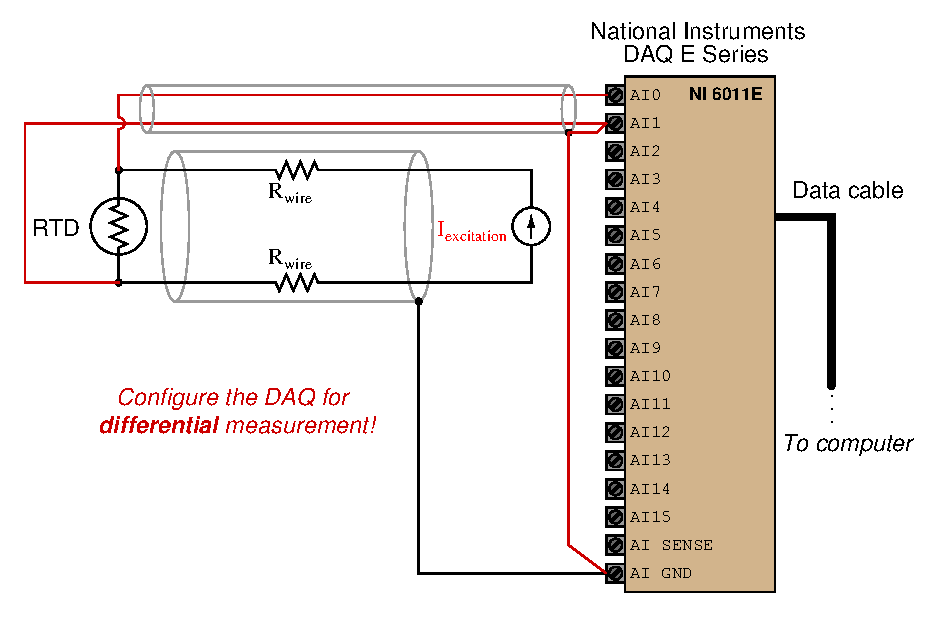
\includegraphics[width=15.5cm]{i02122x02.eps}$$

%(END_ANSWER)





%(BEGIN_NOTES)


%INDEX% Pictorial circuit review (analog signal wiring to data acquisition unit)

%(END_NOTES)


